\documentclass{article}
\usepackage{physics}
\usepackage{graphicx}
\usepackage{caption}
\usepackage{amsmath}
\usepackage{bm}
\usepackage{framed}
\usepackage{authblk}
\usepackage{empheq}
\usepackage{amsfonts}
\usepackage{esint}
\usepackage[makeroom]{cancel}
\usepackage{dsfont}
\usepackage{centernot}
\usepackage{mathtools}
\usepackage{bigints}
\usepackage{amsthm}
\theoremstyle{definition}
\newtheorem{defn}{Definition}[section]
\newtheorem{prop}{Proposition}[section]
\newtheorem{rmk}{Remark}[section]
\newtheorem{thm}{Theorem}[section]
\newtheorem{exmp}{Example}[section]
\newtheorem{prob}{Problem}[section]
\newtheorem{sln}{Solution}[section]
\newtheorem*{prob*}{Problem}
\newtheorem{exer}{Exercise}[section]
\newtheorem*{exer*}{Exercise}
\newtheorem*{sln*}{Solution}
\usepackage{empheq}
\usepackage{tensor}
\usepackage{xcolor}
%\definecolor{colby}{rgb}{0.0, 0.0, 0.5}
\definecolor{MIT}{RGB}{163, 31, 52}
\usepackage[pdftex]{hyperref}
%\hypersetup{colorlinks,urlcolor=colby}
\hypersetup{colorlinks,linkcolor={MIT},citecolor={MIT},urlcolor={MIT}}  
\usepackage[left=1in,right=1in,top=1in,bottom=1in]{geometry}

\usepackage{newpxtext,newpxmath}
\newcommand*\widefbox[1]{\fbox{\hspace{2em}#1\hspace{2em}}}

\newcommand{\p}{\partial}
\newcommand{\R}{\mathbb{R}}
\newcommand{\C}{\mathbb{C}}
\newcommand{\lag}{\mathcal{L}}
\newcommand{\nn}{\nonumber}
\newcommand{\ham}{\mathcal{H}}
\newcommand{\M}{\mathcal{M}}
\newcommand{\I}{\mathcal{I}}
\newcommand{\K}{\mathcal{K}}
\newcommand{\F}{\mathcal{F}}
\newcommand{\w}{\omega}
\newcommand{\lam}{\lambda}
\newcommand{\al}{\alpha}
\newcommand{\be}{\beta}
\newcommand{\x}{\xi}
\def\dbar{{\mkern3mu\mathchar'26\mkern-12mu   d}}


\newcommand{\G}{\mathcal{G}}

\newcommand{\f}[2]{\frac{#1}{#2}}

\newcommand{\ift}{\infty}

\newcommand{\lp}{\left(}
\newcommand{\rp}{\right)}

\newcommand{\lb}{\left[}
\newcommand{\rb}{\right]}

\newcommand{\lc}{\left\{}
\newcommand{\rc}{\right\}}


\newcommand{\V}{\mathbf{V}}
\newcommand{\U}{\mathcal{U}}
\newcommand{\Id}{\mathcal{I}}
\newcommand{\D}{\mathcal{D}}
\newcommand{\Z}{\mathcal{Z}}

%\setcounter{chapter}{-1}



\usepackage{enumitem}


\usepackage{subfig}
\usepackage{listings}
\captionsetup[lstlisting]{margin=0cm,format=hang,font=small,format=plain,labelfont={bf,up},textfont={it}}
\renewcommand*{\lstlistingname}{Code \textcolor{violet}{\textsl{Mathematica}}}
\definecolor{gris245}{RGB}{245,245,245}
\definecolor{olive}{RGB}{50,140,50}
\definecolor{brun}{RGB}{175,100,80}

%\hypersetup{colorlinks,urlcolor=colby}
\lstset{
	tabsize=4,
	frame=single,
	language=mathematica,
	basicstyle=\scriptsize\ttfamily,
	keywordstyle=\color{black},
	backgroundcolor=\color{gris245},
	commentstyle=\color{gray},
	showstringspaces=false,
	emph={
		r1,
		r2,
		epsilon,epsilon_,
		Newton,Newton_
	},emphstyle={\color{olive}},
	emph={[2]
		L,
		CouleurCourbe,
		PotentielEffectif,
		IdCourbe,
		Courbe
	},emphstyle={[2]\color{blue}},
	emph={[3]r,r_,n,n_},emphstyle={[3]\color{magenta}}
}






\begin{document}
		\begin{framed}
			\noindent Name: \textbf{Huan Q. Bui}\\
			Course: \textbf{8.333 - Statistical Mechanics I}\\
			Problem set: \textbf{\#4}
		\end{framed}
	




\noindent \textbf{1. Rotating gas.} The Hamiltonian is 
\begin{align*}
\ham = \sum^N_{n=1} \lb \f{(p^{(n)})^2}{2m} + \f{K}{2} (r^{(n)})^2 \rb
\end{align*}

\begin{enumerate}[label=(\alph*)]
	\item The components of the angular momentum of particle $n$ is $L_i^{(n)} = \epsilon_{ijk} r^{(n)}_j p^{(n)}_k$. To show that $\{ \vec{L}^{(n)},\ham\} = 0$ we may show that $\{ L^{(n)}_i, \ham\} = 0$.
	\begin{align*}
	\{ L_i^{(n)} , \ham\} 
	&= \epsilon_{ijk}\{ r_j^{(n)} p_k^{(n)},  \ham \}\\
	&= \epsilon_{ijk}\{ r_j^{(n)},\ham \}p_k^{(n)} + \epsilon_{ijk} r_j^{(n)} \{ p_k^{(n)},\ham  \}
	\end{align*}
	Since there is no interaction, the only nontrivial Poisson brackets are those with partial derivatives with respect to the canonical variables associated with the particle $(n)$ (we can also show this explicitly by definition but it's just a matter of notation). If we write $\ham = \sum_n^N \ham(n)$ then we have
	\begin{align*}
	\{ L_i^{(n)} , \ham\} 
	&= \epsilon_{ijk}\{ r_j^{(n)},\ham^{(n)} \}p_k^{(n)} + \epsilon_{ijk} r_j^{(n)} \{ p_k^{(n)},\ham^{(n)}  \}\\
	&= \f{1}{2m}\epsilon_{ijk}\{ r_j^{(n)}, p^{(n)}_a p^{(n)}_a  \}p_k^{(n)} + \f{K}{2}\epsilon_{ijk} r_j^{(n)} \{ p_k^{(n)}, r^{(n)}_b r^{(n)}_b  \}\\
	&= -\f{1}{2m}\epsilon_{ijk}\{ p^{(n)}_a p^{(n)}_a , r_j^{(n)} \}p_k^{(n)} - \f{K}{2}\epsilon_{ijk} r_j^{(n)} \{  r^{(n)}_b r^{(n)}_b, p_k^{(n)}  \}\\
	&= -\f{1}{m}\epsilon_{ijk}\{ p^{(n)}_a  , r_j^{(n)} \}  p_a^{(n)} p_k^{(n)} - K\epsilon_{ijk}  \{  r^{(n)}_b , p_k^{(n)}  \} r^{(n)}_b r_j^{(n)}\\
	&= \f{1}{m}\epsilon_{ijk} \delta_{aj} p_a^{(n)}p_k^{(n)} + K\epsilon_{ijk}\delta_{bk}r_b^{(n)}r_j^{(n)}\\
	&= \f{1}{m}\epsilon_{ijk} p_j^{(n)} p_k^{(n)} + K \epsilon_{ijk} r_k^{(n)} r_j^{(n)}\\
	&= 0,
	\end{align*}
	where we have used the fact that $\vec{a}^{(n)} \times \vec{a}^{(n)} = \vec{0}$ for any $\vec{a}^{(n)}$.
	
	
	\item The generalized canonical distribution is 
	\begin{align*}
	p[\mu \equiv \{ \vec{p}_i ,\vec{r}_i \}] = \f{1}{\mathcal{Z}(\be,\vec{\Omega})} \exp\lp -\be \ham(\mu) - \be \vec{\Omega}\cdot \vec{L} \rp 
	\end{align*}
	Assuming that $\vec{\Omega}  =\Omega \hat{z}$ where $\Omega < \sqrt{k/m}$, so that $\vec{\Omega} \cdot \vec{L} = \Omega L_z$, we may compute $\mathcal{Z}$ as follows. 
	\begin{align*}
	\mathcal{Z}(\be,\Omega) 
	&= \f{1}{N! h^{3N}}\int\,d\mu  \exp\lp -\be \ham(\mu) - \be \vec{\Omega}\cdot \vec{L} \rp \\
	&= \f{1}{N! h^{3N}}\prod^N_{n=1} \int\,d\mu^{(n)} \exp\lp -\be \ham^{(n)}(\mu^{(n)})\rp \exp\lp - \beta \Omega L_z^{(n)}  \rp\\
	&= \f{1}{N! h^{3N}}\lb \int d^3 r d^3 p \exp\lp \beta \lp \f{p^2}{2m} + \f{K}{2}r^2 \rp \rp \exp\lp -\be\Omega(xp_y - y p_x)  \rp  \rb^N  \\
	&= \f{1}{N! h^{3N}}\lb \f{8\pi^3 \sqrt{m}}{\sqrt{K}\be^{3}  (K/m-\Omega^2)}\rb^N = \boxed{\f{1}{N! h^{3N}}\lb \f{8\pi^3}{\omega\be^{3}  (\omega^2-\Omega^2)}\rb^N}
	\end{align*}
	where we have called $\omega = \sqrt{K/m}$. Mathematica code:
	\begin{lstlisting}
	Integrate[
	Exp[-\[Beta]*((px^2 + py^2 + pz^2)/(2*m) + K*(x^2 + y^2 + z^2)/2)]*
	Exp[-\[Beta]*\[CapitalOmega]*(x*py - y*px)], {px, -Infinity, 
	Infinity}, {py, -Infinity, Infinity}, {pz, -Infinity, Infinity},
	{x, -Infinity, Infinity}, {y, -Infinity, Infinity}, {z, -Infinity, 
	Infinity}]
	
	>>> ConditionalExpression[(8 \[Pi]^3)/(
	Sqrt[K \[Beta]] (\[Beta]/m)^(5/2)
	Abs[m] Abs[
	K - m \[CapitalOmega]^2]), (m > 0 && Re[\[Beta]] > 0) || (m < 0 && 
	Re[\[Beta]] < 0)]
	\end{lstlisting}
	
	\item By symmetry, $\langle L_z\rangle = \sum^N_{n=1}\langle L_z^{(n)}\rangle = N\langle L_z^{(n)}\rangle$, so 
	\begin{align*}
	\langle L_z \rangle 
	&= \f{N}{\mathcal{Z}(\be,\vec{\Omega})}\int d^3r d^3p (xp_y - yp_x)\exp\lp \beta \lp \f{p^2}{2m} + \f{K}{2}r^2 \rp \rp \exp\lp -\be\Omega(xp_y - y p_x)  \rp  \lb \int d\mu \Pr[\mu] \rb^{N-1}\\
	&= \f{N}{\mathcal{Z}^{1/N}} \int d^3r d^3p (xp_y - yp_x)\exp\lp \beta \lp \f{p^2}{2m} + \f{K}{2}r^2 \rp \rp \exp\lp -\be\Omega(xp_y - y p_x)  \rp \\
	&= \f{N}{\mathcal{Z}^{1/N}} \f{1}{h^3 (N!)^{1/N}} \f{-16m^2 \pi^3 \sqrt{K\be} \Omega}{K\be^4 \sqrt{\be/m} (K-m\Omega)^2}\\
	&= N \f{\omega \be^{3} (\omega^2 - \Omega^2)}{8\pi^3} \f{-16 \pi^3 \Omega}{ \be^4 \omega(\omega^2 - \Omega^2)^2} \\
	&=  \boxed{\f{-2N \Omega}{\be(\omega^2 - \Omega^2)}}
	\end{align*}
	Mathematica code:
	\begin{lstlisting}
	In[6]:= Integrate[(x*py - y*px)*
	Exp[-\[Beta]*((px^2 + py^2 + pz^2)/(2*m) + K*(x^2 + y^2 + z^2)/2)]*
	Exp[-\[Beta]*\[CapitalOmega]*(x*py - y*px)], {px, -Infinity, 
	Infinity}, {py, -Infinity, Infinity}, {pz, -Infinity, Infinity},
	{x, -Infinity, Infinity}, {y, -Infinity, Infinity}, {z, -Infinity, 
	Infinity}]
	
	Out[6]= ConditionalExpression[-((
	16 m^2 \[Pi]^3 Sqrt[K \[Beta]] \[CapitalOmega])/(
	K \[Beta]^4 Sqrt[\[Beta]/m] (K - m \[CapitalOmega]^2)^2)), 
	Re[\[Beta] (1/m - \[CapitalOmega]^2/K)] > 0]
	
	(*Find 1/N * <Lz>*)
	In[16]:= (-((16 m^2 \[Pi]^3 Sqrt[K \[Beta]] \[CapitalOmega])/(
	K \[Beta]^4 Sqrt[\[Beta]/m] (K - m \[CapitalOmega]^2)^2)))/((
	8 \[Pi]^3)/(
	Sqrt[K \[Beta]] (\[Beta]/m)^(5/2)
	Abs[m (K - m \[CapitalOmega]^2)])) // FullSimplify
	
	Out[16]= -((
	2 \[CapitalOmega] Abs[
	m (K - m \[CapitalOmega]^2)])/(\[Beta] (K - m \[CapitalOmega]^2)^2)
	)
	\end{lstlisting}
	
	\item The probability density of finding a particle at location $(x, y, z)$ is taken by integrating out all momentum parts. Since we also don't have interaction, we simply look at one-particle partition function $\mathcal{Z}^{1/N}$ and 1-particle densities only:
	\begin{align*}
	\rho(x,y,z) 
	&= \f{1}{\mathcal{Z}^{1/N}}\lb 
	\int d^3p \exp\lp -\be \f{p^2}{2m} -\be \f{K}{2}(x^2 + y^2 + z^2) - \be \Omega (xp_y - yp_x)\rp \rb\\
	&= \f{1}{\mathcal{Z}^{1/N}}  \f{1}{(N!)^{1/N}h^3} 2\sqrt{2} \pi^{3/2}\lp \f{m}{\be}\rp^{3/2}  \exp\lp -\f{ \be K}{2}(x^2+y^2+z^2) \rp \exp\lp -\Omega^2(x^2+y^2) \rp.
	\end{align*}
	
	Hence, we have 
	\begin{align*}
	&\langle x^2 \rangle = \int x^2 \rho\,dV =  \f{1}{\mathcal{Z}^{1/N}} \f{1}{(N!)^{1/N}h^3}\f{8\pi^3}{\be^2\sqrt{K\be}( \be/m)^{3/2}(K-m\Omega^2)^2}  = \f{1}{\be(K-m\Omega^2)} = \boxed{\f{1}{\be m (\omega^2 - \Omega^2)}}\\
	&\langle y^2 \rangle = \f{1}{\be(K-m\Omega^2)}= \boxed{\f{1}{\be m (\omega^2 - \Omega^2)}} \quad\quad \text{by symmetry}\\
	&\langle z^2 \rangle = \f{1}{\mathcal{Z}^{1/N}}\int z^2 \rho\,dV = \f{1}{\mathcal{Z}^{1/N}} \f{1}{(N!)^{1/N}h^3}\f{8\pi^3}{(K\be)^{3/2}(\be/m)^{3/2}\be (K-m\Omega^2)}   = \boxed{\f{1}{K\be}}
	\end{align*}
	
	Mathematica code:
	\begin{lstlisting}
	(*x^2*)
	In[25]:= Integrate[
	x^2*(2 Sqrt[2]
	E^(-(1/2) \[Beta] (K (x^2 + y^2 + z^2) - 
	m (x^2 + y^2) \[CapitalOmega]^2)) m \[Pi]^(
	3/2))/(\[Beta] Sqrt[\[Beta]/m]), {x, -Infinity, 
	Infinity}, {y, -Infinity, Infinity}, {z, -Infinity, Infinity}]
	
	Out[25]= ConditionalExpression[(
	8 \[Pi]^3)/(\[Beta]^2 Sqrt[K \[Beta]] (\[Beta]/m)^(
	3/2) (K - m \[CapitalOmega]^2)^2), And[
	Or[
	Element[\[Beta] (K - m \[CapitalOmega]^2), Reals], 
	Re[\[Beta] (K - m \[CapitalOmega]^2)] > 0], 
	Re[\[Beta] (K - m \[CapitalOmega]^2)] >= 0, 
	Re[m \[Beta] \[CapitalOmega]^2] < Re[K \[Beta]]]]
	
	(*Simplify for x^2*)
	In[28]:= ((
	8 \[Pi]^3)/(\[Beta]^2 Sqrt[K \[Beta]] (\[Beta]/m)^(
	3/2) (K - m \[CapitalOmega]^2)^2))/((8 \[Pi]^3)/(
	Sqrt[K \[Beta]] (\[Beta]/m)^(5/2)
	Abs[m] Abs[K - m \[CapitalOmega]^2]))
	
	Out[28]= (
	Abs[m] Abs[
	K - m \[CapitalOmega]^2])/(m \[Beta] (K - m \[CapitalOmega]^2)^2)
	
	(*z^2*)
	In[29]:= Integrate[
	z^2*(2 Sqrt[2]
	E^(-(1/2) \[Beta] (K (x^2 + y^2 + z^2) - 
	m (x^2 + y^2) \[CapitalOmega]^2)) m \[Pi]^(
	3/2))/(\[Beta] Sqrt[\[Beta]/m]), {x, -Infinity, 
	Infinity}, {y, -Infinity, Infinity}, {z, -Infinity, Infinity}]
	
	Out[29]= ConditionalExpression[(
	8 \[Pi]^3)/((K \[Beta])^(3/2) (\[Beta]/m)^(
	3/2) (K \[Beta] - m \[Beta] \[CapitalOmega]^2)), 
	Re[\[Beta] (K - m \[CapitalOmega]^2)] > 0]
	
	(*Simplify for z^2*)
	In[31]:= ((
	8 \[Pi]^3)/((K \[Beta])^(3/2) (\[Beta]/m)^(
	3/2) (K \[Beta] - m \[Beta] \[CapitalOmega]^2)))/((8 \[Pi]^3)/(
	Sqrt[K \[Beta]] (\[Beta]/m)^(5/2)
	Abs[m] Abs[K - m \[CapitalOmega]^2]))
	
	Out[31]= (
	Abs[m] Abs[
	K - m \[CapitalOmega]^2])/(K m (K \[Beta] - 
	m \[Beta] \[CapitalOmega]^2))
	\end{lstlisting}
\end{enumerate}


\noindent \textbf{2. Polar rods.} The Hamiltonian is 
\begin{align*}
\ham_\text{rot} = \f{1}{2I}\lp p_\theta^2 + \f{p_\phi^2}{\sin^2\theta} \rp - \mu E \cos\theta. 
\end{align*}

\begin{enumerate}[label=(\alph*)]
	
	
	\item The contribution of the rotational degrees of freedom of each dipole to the
	classical partition function is 
	\begin{align*}
	\mathcal{Z}_\text{rot} 
	&= \f{1}{h^2}\int^{2\pi}_0 d\phi \int^\pi_0 \,d\theta \int dp_\phi\,dp_\theta \exp\lp -\f{\be}{2I} \lp p^2_\theta + \f{p_\phi^2}{\sin^2\theta}\rp + \be E\mu\cos\theta\rp\\
	&= \boxed{\f{8I\pi^2\sinh(\be\mu E)}{Eh^2\be^2 \mu}}
 	\end{align*}
 	Mathematica code:
 	\begin{lstlisting}
 	In[1]:= (1/h^2) Integrate[
 	2*Pi*Exp[-(\[Beta]/(2*II))*(p\[Theta]^2 + 
 	p\[Phi]^2/Sin[\[Theta]]^2) + \[Beta]*Ef*\[Mu]*
 	Cos[\[Theta]]], {\[Theta], 0, Pi}, {p\[Theta], -Infinity, 
 	Infinity}, {p\[Phi], -Infinity, Infinity}]
 	
 	Out[1]= (8 II \[Pi]^2 Sinh[Ef \[Beta] \[Mu]])/(Ef h^2 \[Beta]^2 \[Mu])
 	\end{lstlisting}
	
	\item The mean polarization is 
	\begin{align*}
	P = \langle \mu \cos\theta \rangle = \f{\p}{\p (\be E)}\ln \mathcal{Z}_\text{rot} = \f{\p}{\p (\be E)}\lb \ln \sinh(\be \mu E) - \ln E\be \rb = \boxed{\mu \coth(\be \mu E) - \f{1}{E\be}}
	\end{align*}
	Brute-forcing using the definition (using Mathematica) also works. Mathematica code:
	\begin{lstlisting}
	(1/((8 II \[Pi]^2 Sinh[Ef \[Beta] \[Mu]])/(
	Ef h^2 \[Beta]^2 \[Mu]))) (1/
	h^2) Integrate[(\[Mu]*Cos[\[Theta]])*2*Pi*
	Exp[-(\[Beta]/(2*II))*(p\[Theta]^2 + 
	p\[Phi]^2/Sin[\[Theta]]^2) + \[Beta]*Ef*\[Mu]*
	Cos[\[Theta]]], {\[Theta], 0, Pi}, {p\[Theta], -Infinity, 
	Infinity}, {p\[Phi], -Infinity, Infinity}]
	
	Out[2]= (Csch[
	Ef \[Beta] \[Mu]] (Ef \[Beta] \[Mu] Cosh[Ef \[Beta] \[Mu]] - 
	Sinh[Ef \[Beta] \[Mu]]))/(Ef \[Beta])
	
	In[6]:= (Csch[
	Ef \[Beta] \[Mu]] (Ef \[Beta] \[Mu] Cosh[Ef \[Beta] \[Mu]] - 
	Sinh[Ef \[Beta] \[Mu]]))/(Ef \[Beta]) // FullSimplify
	
	Out[6]= -(1/(Ef \[Beta])) + \[Mu] Coth[Ef \[Beta] \[Mu]]
	\end{lstlisting}
	
	\item The zero-field polarizability is 
	\begin{align*}
	\chi_T = \f{\p P}{\p E}\bigg\vert_{E=0} = \lim_{E\to 0} \lb -\be \mu^2 \csch^2(E\be\mu)  + \f{1}{E^2\be}\rb = \boxed{\f{\be\mu^2}{3}}
	\end{align*}
	where instead of naivly plugging in $E=0$ we have taken the limit $E\to 0$ to get this result. 
	
	Mathematica code:
	\begin{lstlisting}
	In[8]:= D[-(1/(Ef \[Beta])) + \[Mu] Coth[Ef \[Beta] \[Mu]], 
	Ef] // FullSimplify
	
	Out[8]= 1/(Ef^2 \[Beta]) - \[Beta] \[Mu]^2 Csch[Ef \[Beta] \[Mu]]^2
	
	In[9]:= Limit[
	1/(Ef^2 \[Beta]) - \[Beta] \[Mu]^2 Csch[Ef \[Beta] \[Mu]]^2, Ef -> 0]
	
	Out[9]= (\[Beta] \[Mu]^2)/3
	\end{lstlisting}
	
	\item The rotational energy per particle for a given $E$ is 
	\begin{align*}
	\langle E_\text{rot}\rangle = -\f{\p}{\p \be}\ln \mathcal{Z}_\text{rot} = \boxed{\f{2}{\be} - E\mu\coth(E\mu\be)}
	\end{align*}
	
	Mathematica code:
	\begin{lstlisting}
	In[11]:= -D[
	Log[(8 II \[Pi]^2 Sinh[Ef \[Beta] \[Mu]])/(
	Ef h^2 \[Beta]^2 \[Mu])], \[Beta]] // FullSimplify
	
	Out[11]= 2/\[Beta] - Ef \[Mu] Coth[Ef \[Beta] \[Mu]]
	\end{lstlisting}
	
	To see what $\langle E_\text{rot}\rangle$ behaves like in the high/low temperature limits we may write it more explicitly:
	\begin{align*}
	\langle E_\text{rot}\rangle = 2k_BT -E\mu \f{e^{2E\mu/k_BT} + 1}{e^{2E\mu/k_BT} - 1}.
	\end{align*}
	In the high temperature limit, $\boxed{\langle E_\text{rot}\rangle \sim 2k_BT}$, while in the low temperature limit $\boxed{\langle E_\text{rot}\rangle \sim   2k_BT - E\mu   }$.
	
	\item Heat capacity is 
	\begin{align*}
	C = \f{d\langle E_\text{rot}\rangle}{dT} = 2k_B - \f{E^2\mu^2}{k_BT^2}\csch\lp \f{E\mu}{k_BT} \rp = 2k_B - \f{E^2\mu^2}{k_BT^2}\f{2e^{E\mu/k_BT}}{e^{2E\mu/k_BT}-1}.
	\end{align*}
	We find 
	\begin{align*}
	&\lim_{T\to 0} C = 2k_B \\
	&\lim_{T\to \infty} C = k_B.
	\end{align*}
	Mathematica code:
	\begin{lstlisting}
	In[30]:= Limit[2 k - (Ef^2 \[Mu]^2 Csch[(Ef \[Mu])/(k T)]^2)/(k T^2), 
	T -> 0]
	
	Out[30]= ConditionalExpression[2 k, Ef k \[Mu] > 0]
	
	In[31]:= Limit[2 k - (Ef^2 \[Mu]^2 Csch[(Ef \[Mu])/(k T)]^2)/(k T^2), 
	T -> Infinity]
	
	Out[31]= k
	\end{lstlisting}
	
	
	Sketch of rotational heat capacity per dipole. Setting $k_B = 1$:
	\begin{figure}[!htb]
		\centering
		\includegraphics[width=0.5\textwidth]{problem2.eps}
	\end{figure}
	The point where the curve begins to decrease fast is where $k_BT \approx E\mu$.

	Mathematica code:
	\begin{lstlisting}
	Plot[2 - Csch[1/T]^2/T^2, {T, 0, 6}, PlotRange -> Full]
	\end{lstlisting}
	
\end{enumerate}



\noindent \textbf{3. Atomic/molecular hydrogen.}

\begin{enumerate}[label=(\alph*)]
	\item Given $N_1$ hydrogen atoms with
	\begin{align*}
	\ham_a = \sum^{N_1}_{i=1} \f{p_i^2}{2m}
	\end{align*}
	the partition function $\mathcal{Z}_a(N_1,T,V)$ is 
	\begin{align*}
	\mathcal{Z}_a(N_1,T,V) = \f{V^{N_1}}{N_1!h^{3N_1}}\lb \int \exp(-\be \f{p^2}{2m}) \,d^3p\rb^{N_1} = \boxed{{\f{V^{N_1}}{N_1! h^{3N_1}} \lp \f{2\pi m}{\be} \rp^{3N_1/2}}}
	\end{align*}
	
	\item Given 
	\begin{align*}
	\ham_m = \sum_{i=1}^{N_2} \lb \f{p_i^2}{4m} + \f{L_i^2}{2I} -\epsilon  \rb = \sum_{i=1}^{N_2} \lb \f{(p^{(i)})^2}{4m} + \f{1}{2I}\lp (p^{(i)}_\theta)^2 + \f{(p^{(i)}_\phi)^2}{\sin^2\theta} \rp -\epsilon  \rb
	\end{align*}
	in view of the previous problem. The external and internal degrees of freedom of the molecule completely decouple. Also, the extra factor of $\exp(\be\epsilon)$ simply carries along. So, we have
	\begin{align*}
	\mathcal{Z}_m(N_2,T,V) = {\f{V^{N_2}}{N_2! h^{3N_2}} \lp \f{4\pi m}{\be} \rp^{3N_2/2}} e^{N_2\be\epsilon} \mathcal{Z}_\text{rot}
	\end{align*}
	where
	\begin{align*}
	\mathcal{Z}_\text{rot} 
	= 
	 \f{1}{h^{2N_2}}\lc \int^{2\pi}_0 d\phi \int^\pi_0 d\theta \int dp_\phi\,dp_\theta \exp\lb -\f{\be}{2I} \lp p^2_\theta + \f{p_\phi^2}{\sin^2\theta}\rp \rb \rc^{N_2}
	=\lp\f{8I\pi^2}{h^2\be}\rp^{N_2}
	\end{align*}
	Mathematica code:
	\begin{lstlisting}
	In[1]:= Integrate[
	2*Pi*Exp[(-\[Beta]/(2*II))*(p\[Theta]^2 + 
	p\[Phi]^2/Sin[\[Theta]]^2)], {\[Theta], 0, 
	Pi}, {p\[Theta], -Infinity, Infinity}, {p\[Phi], -Infinity, 
	Infinity}]
	
	Out[1]= (8 II \[Pi]^2)/\[Beta]
	\end{lstlisting}
	
	So we have
	\begin{align*}
	\mathcal{Z}_m(N_2,T,V) = \boxed{{\f{V^{N_2}}{N_2! h^{3N_2}} \lp \f{4\pi m}{\be} \rp^{3N_2/2}}  \lp\f{8I\pi^2}{h^2\be}\rp^{N_2}e^{N_2\be\epsilon}}
	\end{align*}
	
	
	
	\item At equilibrium, the free energy is extremized. This implies that $\mathcal{Z}_a\mathcal{Z}_m$ is extremized i.e. $\ln \mathcal{Z}_a + \ln \mathcal{Z}_m$ is extremized (since the log is a monotically increasing function). Using the Stirling approximation we find 
	\begin{align*}
	&\ln \mathcal{Z}_a  = -N_1 \ln N_1 + \ln \f{V^{N_1}}{h^{3N_1}} + \f{3N_1}{2}\log \f{2\pi m }{\be}\\
	&\ln \mathcal{Z}_m  = -N_2\ln N_2  + \ln \f{V^{N_2}}{h^{3N_2}} + \f{3N_2}{2}\log \f{4\pi m }{\be} + N_2\log \lb \f{8I\pi^2}{h^2\be} e^{\be\epsilon} \rb.
	\end{align*}
	Setting $N_2 = (N-N_1/2)$ and writing
	\begin{align*}
	\f{\p}{\p N_1}\lb  \ln \mathcal{Z}_a + \ln \mathcal{Z}_m \rb = 0
	\end{align*}
	gives us 
	\begin{align*}
	\ln \lb \f{2n_m}{n_a^2} \rb = \ln \lb \f{2N_2 V}{N_1^2} \rb = \ln \lb \f{(N-N_1)V}{N_1^2} \rb = 1 + 3\ln h + \f{1}{2}\ln (256\pi) + \f{3}{2}\ln (k_B m T) - \ln \lp \f{I k_BT e^{\epsilon/k_BT}}{h^2} \rp
	\end{align*}
	And so we have
	\begin{align*}
	\boxed{\f{n_m}{n_a^2} = \f{8\sqrt{\pi} hI  }{m^{3/2} \sqrt{k_BT}} e^{1+\epsilon/k_BT}}
	\end{align*}
	Mathematica code:
	\begin{lstlisting}
	In[52]:= A = (8 II \[Pi]^2)/(h^2*\[Beta])*Exp[\[Beta]*e];
	
	In[56]:= N2 = (n - N1)/2;
	
	In[57]:= D[-N1*Log[N1] + 
	Log[V^N1/(h^(3*N1))] + (3*N1/2) Log[2*Pi*m*k*T]
	- N2*Log[N2] + Log[V^N2/(h^(3*N2))] + (3*N2/2)*Log[2*2*Pi*m*k*T] + 
	N2*Log[A], N1] // FullSimplify
	
	Out[57]= 1/4 (-2 - 6 Log[h] + 2 Log[n - N1] - 4 Log[N1] - 
	Log[256 \[Pi]] + 3 Log[k m T] + 2 Log[V] - 
	2 Log[(E^(e \[Beta]) II)/(h^2 \[Beta])])
	
	In[62]:= B = -1 - 
	3 Log[h] - (1/2) Log[256 \[Pi]] + (3/2) Log[k m T] - 
	Log[(E^(e \[Beta]) II)/(h^2 \[Beta])];
	
	In[63]:= (1/2)*Exp[-B] /. {\[Beta] -> 1/(k*T)} // FullSimplify
	
	Out[63]= (8 E^(1 + e/(k T)) h II k Sqrt[\[Pi]] T)/(k m T)^(3/2)
	\end{lstlisting}
\end{enumerate}



\noindent \textbf{4. Fluctuation-induced dipole interactions.}

\begin{enumerate}[label=(\alph*)]
	\item We may rewrite $V(r)$ as 
	\begin{align*} 
	V(r) 
	&= \f{1}{r^3} \lb 3D_1 D_2 \cos\theta_1 \cos\theta_2  - \vec{D_1} \cdot \vec{D_2} \rb
 	\end{align*}
 	putting things in coordinate form we have
 	\begin{align*}
 	V(r) = \f{D_1 D_2}{r^3}\lb 2\cos\theta_1 \cos\theta_2 - \sin\theta_1\sin\theta_2\cos(\phi_1 - \phi_2) \rb
 	\end{align*}
 	where I have used the fact that
 	\begin{align*}
 	\vec{D}_1 \cdot \vec{D_2} = D_1D_2 (\cos\theta_1\cos\theta_2 + \sin\theta_1\sin\theta_2\cos(\phi_1-\phi_2))
 	\end{align*}
 	when writing $\vec{D}_1$ and $\vec{D}_2$ in spherical coordinates.  With this we can calculate the partition function as follows (ignoring factors of $h$ for now):
 	\begin{align*}
	\mathcal{Z}(r) = \int_0^{2\pi}\,d\phi_1 \int_0^{2\pi}\,d\phi_2 \int_0^\pi \sin\theta_1 \, d\theta_1 \int_0^\pi \sin\theta_2\, d\theta_2 \exp(-\be V) 
	\end{align*}
	Expanding 
	\begin{align*}
	\exp(\be V) \approx 1 - \be V + \f{1}{2}\be^2 V^2 + \dots 
	\end{align*}
	we get
	\begin{align*}
	\boxed{\mathcal{Z}(r) \approx 16\pi^2 + \f{16\pi^2}{3}D_1^2D_2^2 \f{\beta^2}{r^6} + \dots}
	\end{align*}
	Mathematica code:
	\begin{lstlisting}
	(*D1 dot D2*)
	In[28]:= v1 = {D1*Sin[\[Theta]1]*Cos[\[Phi]1], 
	D1*Sin[\[Theta]1]*Sin[\[Phi]1], D1*Cos[\[Theta]1]}
	
	Out[28]= {D1 Cos[\[Phi]1] Sin[\[Theta]1], 
	D1 Sin[\[Theta]1] Sin[\[Phi]1], D1 Cos[\[Theta]1]}
	
	In[29]:= v2 = {D2*Sin[\[Theta]2]*Cos[\[Phi]2], 
	D2*Sin[\[Theta]2]*Sin[\[Phi]2], D2*Cos[\[Theta]2]}
	
	Out[29]= {D2 Cos[\[Phi]2] Sin[\[Theta]2], 
	D2 Sin[\[Theta]2] Sin[\[Phi]2], D2 Cos[\[Theta]2]}
	
	In[31]:= Dot[v1, v2] // FullSimplify
	
	Out[31]= D1 D2 (Cos[\[Theta]1] Cos[\[Theta]2] + 
	Cos[\[Phi]1 - \[Phi]2] Sin[\[Theta]1] Sin[\[Theta]2])
	
	(*First order*)
	In[33]:= (*First order*)
	
	In[34]:= Integrate[Sin[\[Theta]1]*Sin[\[Theta]2]*\[Beta] (D1*D2)/(R^3)*(2*Cos[\[Theta]1]*
	Cos[\[Theta]2] - 
	Sin[\[Theta]1]*Sin[\[Theta]2]*
	Cos[\[Phi]1 - \[Phi]2] ), {\[Theta]1, 0, Pi}, {\[Theta]2, 0, 
	Pi}, {\[Phi]1, 0, 2 Pi}, {\[Phi]2, 0, 2 Pi}]
	
	Out[34]= 0
	
	(*Second order*)
	In[32]:= (*Second order*)
	
	In[25]:= Integrate[Sin[\[Theta]1]*Sin[\[Theta]2]*(\[Beta]^2/
	2)*(D1*D2)^2/(R^6)*(2*Cos[\[Theta]1]*Cos[\[Theta]2] - 
	Sin[\[Theta]1]*Sin[\[Theta]2]*
	Cos[\[Phi]1 - \[Phi]2] )^2, {\[Theta]1, 0, Pi}, {\[Theta]2, 0, 
	Pi}, {\[Phi]1, 0, 2 Pi}, {\[Phi]2, 0, 2 Pi}]
	
	Out[25]= (16 D1^2 D2^2 \[Pi]^2 \[Beta]^2)/(3 R^6)
	\end{lstlisting}
	
	\item From $\mathcal{Z}(r)$ we can find $U(r)$ as follows. Schematically we have
	\begin{align*}
	\mathcal{Z}(r) = \int \exp(-\be U(r)) = \int d\Omega [1-\be U(r)] = 16\pi^2 [1-\be U(r)]
	\end{align*}
	we can now read off 
	\begin{align*}
	U(r) = -\f{1}{\be} \f{1}{3} D_1^2 D_2^2 \f{\be^2}{r^6} = \boxed{ -\f{D_1^2 D_2^2 }{3k_BT r^6 }} 
	\end{align*}
	
	\item For this problem we just repeat the computation, but also integrating over $D_1, D_2$ with extra Boltzmann weights $\exp[-\be(D_1^2/2\chi_1 + D_2^2/2\chi_2)]$: 
	\begin{align*}
	\mathcal{Z}'(r) &= \int_0^\infty d D_1\int_0^\infty dD_2\int_0^{2\pi}\,d\phi_1 \int_0^{2\pi}\,d\phi_2 \\
	&\quad\int_0^\pi \sin\theta_1 \, d\theta_1 \int_0^\pi \sin\theta_2\, d\theta_2 \exp(-\be V) \exp[-\be(D_1^2/2\chi_1 + D_2^2/2\chi_2)]
	\end{align*}
	where now we no longer treat $D_1,D_2$ as constants. Letting Mathematica do the work we get to low order
	\begin{align*}
	\mathcal{Z}'(r) \approx \f{8\pi^3 \sqrt{\chi_1\chi_2}}{\be } + \f{8\pi^3 (\chi_1\chi_2)^{3/2}}{3\be r^6} + \dots \approx \boxed{ \f{8\pi^3 \sqrt{\chi_1\chi_2}}{\be }\lp 1 + \f{\chi_1\chi_2}{3r^6} \rp}
	\end{align*}
	
	
	
	\item Using the same approach as before, we write
	\begin{align*}
	\mathcal{Z}'(r) = \int d\Omega \,dD_1 dD_2\, \exp(-D_1^2/2\chi_1)\exp(-D_2^2/2\chi_2)\exp(-\be V) = \f{8\pi^3 \sqrt{\chi_1\chi_2}}{\be }\lb 1- \be U'(r) \rb
	\end{align*}
	
	from which we can read off the effective potential:
	\begin{align*}
	U'(r) = -\f{1}{\be} \f{\chi_1\chi_2}{3r^6} = \boxed{-k_BT \f{\chi_1\chi_2}{3r^6}}
	\end{align*}
	Mathematica code:
	\begin{lstlisting}
	Z0=Integrate[Sin[\[Theta]1]*Sin[\[Theta]2]*Exp[-\[Beta]*D1^2/(2*\[Chi]1)]*Exp[-\[Beta]*D2^2/
	(2*\[Chi]2)],{D1,0,Infinity},{D2,0,Infinity},{\[Theta]1,0,Pi},{\[Theta]2,0,Pi},{\[Phi]1,0,
	2*Pi},{\[Phi]2,0,2*Pi}]
	
	ConditionalExpression[(8 \[Pi]^3 Sqrt[\[Beta]/\[Chi]2] \[Chi]2^2)/(
	3 r^6 (\[Beta]/\[Chi]1)^(3/2)), Re[\[Beta]/\[Chi]1] > 0]
	
	Z2=Integrate[Sin[\[Theta]1]*Sin[\[Theta]2]*Exp[-\[Beta]*D1^2/(2*\[Chi]1)]*Exp[-\[Beta]*D2^2/(2*\[Chi]2)]
	*(D1*D2)^2*(\[Beta]^2/2)*(2*Cos[\[Theta]1]*Cos[\[Theta]2]-Sin[\[Theta]1]
	*Sin[\[Theta]2]*Cos[\[Phi]1-\[Phi]2])^2/r^6,{D1,0,Infinity}
	,{D2,0,Infinity},{\[Theta]1,0,Pi},{\[Theta]2,0,Pi},{\[Phi]1,0,2*Pi},{\[Phi]2,0,2*Pi}]//FullSimplify
	
	ConditionalExpression[(8 \[Pi]^3 Sqrt[\[Chi]1 \[Chi]2])/\[Beta], 
	Re[\[Beta]] > 0]
	\end{lstlisting}
\end{enumerate}



\noindent \textbf{5. Molecular adsorption.}

\begin{enumerate}[label=(\alph*)]
	\item The smallest energy is attained whenever all molecules lie on the $xy$ plane. Each molecule has two choices for its alignment. With $N$ molecules, there are $\boxed{2^N}$ choices for which the  energy is minimal, $E_\text{min} = 0$. \\
	
	The largest microstate energy is attained whenever all molecules are aligned in the $z$-direction. The energy associated with this microstate is $\boxed{E_\text{max} = N\epsilon}$. 
	
	\item The total energy is $E = N_z \epsilon$ where $N_z$ is the number of molecules aligned in the $z$-direction. This leaves $N - N_z$ molecules in the $xy$ plane. The number of microcanonical microstates is obtained by counting how many ways we could pick $N_z$ molecules out of $N$ molecules, multiplied the number of ways to configure the $N-N_z$ molecules on the $xy$ plane, which is $2^{N-N_z}$.  
	\begin{align*}
	\Omega(E,N) = {N\choose {N_z}} 2^{N-N_z} = \boxed{\f{N!}{N_z! (N  - N_z)!}2^{N-N_z}}
	\end{align*}
	The entropy is given by 
	\begin{align*}
	S(E,N) 
	&= k_B \ln \Omega(E,N) \\
	&= k_B \ln \f{N!}{N_z! (N-N_z)!} + k_B (N-N_z) \ln 2.
	\end{align*}
	We recognize that the first term is simply the entropy for a two-level system (Eq. 4.18 in our textbook), so using Stirling's approximation and using $N_z = E/\epsilon$ we find 
	\begin{align*}
	\boxed{S(E,N) = -Nk_B \lb \f{E}{N\epsilon}  \ln \f{E}{N\epsilon} + \lp 1 - \f{E}{N\epsilon} \rp \ln \lp 1 - \f{E}{N\epsilon} \rp\rb  + k_B \lp N - \f{E}{\epsilon} \rp \ln 2}
	\end{align*}
	
	\item To find what the heat capacity is we must first find the energy as a function of temperature via the entropy. We know that $\p E/ \p S = T$ so inverting gives $\p S/\p E = 1/T$. So, 
	\begin{align*}
	\f{1}{T} = \f{\p S}{\p E} = \f{k_B}{\epsilon}\lb \log \lp 1  - \f{E}{N\epsilon}  \rp - \log \lp \f{2 E}{N\epsilon} \rp  \rb
	\end{align*}
	from which we find 
	\begin{align*}
	E(T) = \f{N\epsilon}{1 + 2e^{\epsilon/k_BT}}.
	\end{align*}
	The heat capacity is given by 
	\begin{align*}
	C = \f{dE}{dT} = \boxed{\f{2N\epsilon^2}{k_B}\f{e^{\epsilon/k_BT}}{T^2\lp 1 +  2 e^{\epsilon/k_BT} \rp^2}}
	\end{align*}
	Letting $x = \epsilon/k_BT$ then we can write
	\begin{align*}
	\f{C(x)}{2k_BN} = x^2\f{e^x}{(1+2e^x)^2}.
	\end{align*}
	Now we can sketch:
	\begin{figure}[!htb]
		\centering
		\includegraphics[width=0.5\textwidth]{problem3.eps}
	\end{figure}



	Mathematica code:
	\begin{lstlisting}
	In[33]:= S = -N*
	k*((En/(N*e))*Log[En/(N*e)] + (1 - En/(N*e))*Log[1 - En/(N*e)]) + 
	k*(N - En/e)*Log[2];
	
	In[36]:= D[S, En] // FullSimplify
	
	Out[36]= (k (Log[1 - En/(e N)] - Log[(2 En)/(e N)]))/e
	
	In[37]:= Solve[
	1/T == (k (Log[1 - En/(e N)] - Log[(2 En)/(e N)]))/e, En]
	
	Out[37]= {{En -> (e N)/(1 + 2 E^(e/(k T)))}}
	
	In[42]:= HC = D[(e N)/(1 + 2 E^(e/(k T))), T] // FullSimplify
	
	Out[42]= (2 e^2 E^(e/(k T)) N)/(k (T + 2 E^(e/(k T)) T)^2)
	
	(*Plotting*)
	In[48]:= Plot[x^2*Exp[x]/(1 + 2*Exp[x])^2, {x, 0, 10}, 
	AxesLabel -> {\[Epsilon]/kT, C/(2 kN)}]
	\end{lstlisting}
	
	\item There are $N_z$ molecules that are standing up, so the probability that any specific molecule is standing up is simply $N_z/N$:
	\begin{align*}
	\boxed{\Pr = \f{N_z}{N}  =\f{E}{N\epsilon} = \f{1}{1 + 2e^{\epsilon/k_BT}}}
	\end{align*}
	
	\item Since the heat capacity is positive for all $T>0$, the energy $E(T)$ is always increasing as $T\to \infty$. However, it turns out that $E$ approach as a limit:
	\begin{align*}
	\boxed{E_\text{max} = \lim_{T\to \infty} \f{N\epsilon}{1 + 2e^{\epsilon/k_BT}} = \f{N\epsilon}{3}}
	\end{align*}
\end{enumerate}




\noindent \textbf{6. Curie susceptibility.}

\begin{enumerate}[label=(\alph*)]
	\item In general, the Gibbs partition function is given by 
	\begin{align*}
	\mathcal{Z}(N,T,B) 
	&= \sum \exp(\be\vec{B}\cdot \vec{M}) \\
	&= \sum_{\text{states}} \exp\lp \be \mu B\sum_{i=1}^N m_i\rp \\
	&= \lb \sum_{m_i = -s,\dots , s} \exp\lp \be \mu B m_i\rp \rb^N\\
	&= {Z}^N
	\end{align*}
	Now we want to evaluate what each $Z$ is:
	\begin{align*}
	Z 
	&= \exp(\be\mu B (-s)) + \exp(\be\mu B (-s+1)) + \dots + \exp(\be\mu B s)\\ 
	&= \exp(\be\mu B (-s))\lb 1 + \exp(\be\mu B) + \exp(2\be\mu B) + \dots + \exp(2\be\mu s) \rb\\
	&= \exp(\be\mu B (-s)) \f{1 - \exp((2s+1)\be\mu B)}{1-\exp(\be\mu B)} \\
	&= \f{\exp(-\be\mu Bs) - \exp(\be\mu B(s+1))}{1-\exp(\be\mu B)}.
	\end{align*}
	So, 
	\begin{align*}
	\boxed{\mathcal{Z}(N,T,B) = \lb \f{\exp(-\be\mu Bs) - \exp(\be\mu B(s+1))}{1-\exp(\be\mu B)}\rb^N}
	\end{align*}
	
	
	\item The Gibbs free energy is 
	\begin{align*}
	\boxed{G = -k_B T \ln \mathcal{Z} = -k_B T N\ln \lb \cosh(s \be\mu B) + \coth(\f{\be\mu B}{2})\sinh(\be\mu B s) \rb}
	\end{align*}
	Mathematica code:
	\begin{lstlisting}
	In[62]:= Z = (Exp[-\[Beta]*\[Mu]*B*s] - 
	Exp[\[Beta]*\[Mu]*B*(s + 1)])/(1 - Exp[\[Beta]*\[Mu]*B]);
	
	In[63]:= G = -kB*T*Log[Z];
	
	In[65]:= G // FullSimplify
	
	Out[65]= -kB T Log[
	Cosh[B s \[Beta] \[Mu]] + 
	Coth[(B \[Beta] \[Mu])/2] Sinh[B s \[Beta] \[Mu]]]
	\end{lstlisting}
	
	
	To obtain $G$ for small $B$, we may Taylor-expand $G$ in powers of $B$ near $B=0$ in Mathematica. The result is 
	\begin{align*}
	G(B) \approx -k_B T N\ln (1+2s) -\f{N}{6} B^2 \lb k_B s (1+s) T \be^2 \mu^2  \rb  + \mathcal{O}(B)^4
	\end{align*}
	Mathematica code:
	\begin{lstlisting}
	In[68]:= Series[G, {B, 0, 3}] // FullSimplify
	
	Out[68]= SeriesData[B, 0, {-kB T Log[1 + 2 s], 0, 
	Rational[-1, 6] kB s (1 + s) T \[Beta]^2 \[Mu]^2}, 0, 4, 1]
	\end{lstlisting}
	
	Notice that
	\begin{align*}
	G(B=0) = \lim_{B \to 0} -k_B T N\ln \lb \cosh(s \be\mu B) + \coth(\f{\be\mu B}{2})\sinh(\be\mu B s) \rb = -k_B T N\ln (1+2s).
	\end{align*}
	Mathematica code:
	\begin{lstlisting}
	In[69]:= Limit[(Exp[-\[Beta]*\[Mu]*B*s] - 
	Exp[\[Beta]*\[Mu]*B*(s + 1)])/(1 - Exp[\[Beta]*\[Mu]*B]), B -> 0]
	
	Out[69]= 1 + 2 s
	\end{lstlisting}
	
	Therefore, we have
	\begin{align*}
	\boxed{G(B) \approx G(0) - \f{N \mu^2 B^2 s(1+s) }{6 k_BT} + \mathcal{O}(B^4)}
	\end{align*}
	as desired. 
	
	
	\item \textbf{\textcolor{blue}{I believe we actually want to calculate $\chi = \p \langle M_z \rangle / \p B$, since otherwise if we stay with the definition in the problem then we don't get $B$-dependence.}} With this, let us calculate $\langle M_z \rangle$ by following the steps in the textook:
	\begin{align*}
	\langle M_z \rangle = \bigg\langle \sum_{i=1}^N m_i \bigg\rangle   = \f{1}{\be}\f{\p}{\p B}\ln \mathcal{Z} = \f{\p}{\p B} (k_BT \ln\mathcal{Z}) = -\f{\p G}{\p B}.
	\end{align*}
	With this, 
	\begin{align*}
	\chi = \f{\p \langle M_z \rangle}{\p B}\bigg\vert_{B=0} = -\f{\p^2 G}{\p B^2}\bigg\vert_{B=0} \approx \boxed{\f{N\mu^2s(1+s)}{3k_BT}}
	\end{align*}
	which is consistent with Curie's law: $\chi = c/T$ where $c = N\mu^2s(1+s)/3k_B$.
	
	\item By definition, 
	\begin{align*}
	C_B - C_M = -B\f{\p \langle M_z\rangle}{\p T}  = \lp \f{N \mu^2 s(1+s)}{3k_B} \rp \f{B^2}{T^2} = \f{cB^2}{T^2}
	\end{align*}
	as desired, where we have used the fact that the magnetic field $B$ is independent of temperature $T$. 
	
	Mathematica code:
	\begin{lstlisting}
	In[75]:= GB = G0 - N*\[Mu]^2*B^2*s (1 + s)/(6*kB*T)
	
	Out[75]= G0 - (B^2 N s (1 + s) \[Mu]^2)/(6 kB T)
	
	In[77]:= -B*D[-D[GB, B], T] // FullSimplify
	
	Out[77]= (B^2 N s (1 + s) \[Mu]^2)/(3 kB T^2)
	\end{lstlisting}
\end{enumerate}


\noindent \textbf{7. Langmuir isotherms.}


\begin{enumerate}[label=(\alph*)]
	\item Following pages 114-115 of the textbook we may use $\lambda(T) = h / \sqrt{2\pi m k_B T}$
	\begin{align*}
	\mu = k_BT\ln \lp \f{N}{V}\lambda^3\rp = k_BT \ln \lb \f{P}{k_BT} \f{h^3}{(2\pi m k_B T)^{3/2}}\rb = \boxed{k_BT\lb  \ln (PT^{-5/2}) + \underbrace{\ln \lp \f{h^3}{k_B^{5/2}(2\pi m)^{3/2}} \rp}_{A_0} \rb}
	\end{align*}
	
	\item The grand partition function is a weighted sum over all microstates. Given $\mathcal{N}$ sites, we must choose $N$ sites which will receive a gas particle. The weight associated with this assignment is $\exp(-\be \epsilon N) \exp(\be\mu N)$. Then, we have to sum over all possible configurations:
	\begin{align*}
	\mathcal{Q} = \sum_{N=0}^\mathcal{N} {\mathcal{N}\choose N} e^{-\be \epsilon N}e^{\be\mu N} = \boxed{\lb 1 + e^{\be(\mu-\epsilon)} \rb^\mathcal{N}}
	\end{align*}
	where we have used the fact that this is simply a binomial expansion.
	
	\item The fraction of occupied surface sites is 
	\begin{align*}
	f = \f{\langle N \rangle }{\mathcal{N}} = \f{1}{\be\mathcal{N}}\f{\p}{\p \mu}\ln \mathcal{Q}  = \f{1}{1 + e^{\be(\epsilon-\mu)}} = \f{1}{1 + e^{\be\epsilon}e^{-\be\mu}}
	\end{align*}
	where we have followed Eq 4.103 in the textbook. Mathematica code:
	\begin{lstlisting}
	In[82]:= (1/(\[Beta]*N))*
	D[Log[(1 + E^(\[Beta] (-\[Epsilon] + \[Mu])))^
	N], \[Mu]] // FullSimplify
	
	Out[82]= 1/(1 + E^(\[Beta] (\[Epsilon] - \[Mu])))
	\end{lstlisting}
	
	
	
	Now, since the gas and the surface has the same temperature and chemical potential we have
	\begin{align*}
	e^{-\be\mu} = \lp\f{N}{V}\lambda^3\rp^{-1} = \f{k_BT}{P\lambda^3}.
	\end{align*}
	With this, we find 
	\begin{align*}
	\boxed{f = f(T,P) = \f{1}{1+e^{\be\epsilon} \f{k_BT}{P\lambda^3}} = \f{P}{P+ P_0(T)}}
	\end{align*}
	where
	\begin{align*}
	\boxed{P_0(T) = \f{k_BT}{\lambda^3}e^{\epsilon/k_BT}}
	\end{align*}
	
	
	
	\item 
	\begin{align*}
	\langle e^{-ikN} \rangle = \f{1}{\mathcal{Q}(\be\mu)}\lb 1 + e^{\be(\mu - \epsilon)} e^{-ik} \rb^\mathcal{N}  = \f{\mathcal{Q}(\be\mu - ik)}{\mathcal{Q}(\be\mu)}.
	\end{align*}
	With this, 
	\begin{align*}
	\langle \mathcal{N}^m \rangle_c &= \f{\p^m}{\p (-ik)^m} \ln \f{\mathcal{Q}(\be\mu - ik)}{\mathcal{Q}(\be\mu)}\\
	&= \f{\p^m}{\p (-ik)^m} \ln {\mathcal{Q}(\be\mu - ik)}\\
	&= \f{\p^m}{\p (-ik)^m} \lb -\be \mathcal{G}(\be\mu - ik)\rb
	\end{align*}
	where we have used Eq. 4.105 in the textbook, with $\mathcal{G}$ denoting the grand potential. With this, we find 
	\begin{align*}
	\langle \mathcal{N}^m \rangle_c 
	= -\be \f{\p^m}{\p (\be\mu)^m}\mathcal{G}(\be\mu - ik)\bigg\vert_T 
	= -\be^{1-m} \f{\p^m \mathcal{G}}{\p \mu^m}\bigg\vert_T 
	= \boxed{-(k_BT)^{m-1}\f{\p^m \mathcal{G}}{\p \mu^m} \bigg\vert_T}
	\end{align*}
	
	\item Setting $m=2$ we find 
	\begin{align*}
	\langle N^2 \rangle_c = -k_BT \f{\p^2 \mathcal{G}}{\p \mu^2}\bigg\vert_T.
	\end{align*}
	Observe that 
	\begin{align*}
	\langle N\rangle = \f{1}{\be}\p_\mu \ln \mathcal{Q} = \f{-\be}{\be}\p_\mu \mathcal{G} = -\f{\p \mathcal{G}}{\p \mu}.
	\end{align*}
	We thus find 
	\begin{align*}
	\boxed{\langle N^2\rangle_c = k_BT \f{\p \langle N \rangle }{\p \mu}\bigg\vert_T}
	\end{align*}
	
	\item We just calculate away...
	\begin{align*}
	\f{\langle N^2\rangle_c}{\langle N\rangle_c^2} 
	&= \f{\langle N^2\rangle_c}{\langle N\rangle^2} \\
	&= \f{k_BT \p_\mu \langle N \rangle}{\mathcal{N}^2 f^2}\bigg\vert_T \\
	&= \f{k_BT}{\mathcal{N}^2 f^2}\lp  \f{\p}{\p \mu} \f{\mathcal{N}}{1 + e^{\be\epsilon - \be\mu} }\rp \bigg\vert_T\\
	&= \f{1}{\mathcal{N} f^2} \f{e^{\be(\epsilon-\mu)}}{(e^{\be\epsilon} + e^{\be\mu})^2}\bigg\vert_T \\
	&= \f{1}{\mathcal{N}f^2} \lb \f{1}{1 + e^{\be\epsilon}e^{-\be\mu}} \lp 1- \f{1}{1 + e^{\be\epsilon}e^{-\be\mu}} \rp \rb\bigg\vert_T \\
	&= \f{f(1-f)}{\mathcal{N} f^2} \\
	&= \boxed{\f{1-f}{\mathcal{N}f}}
	\end{align*}
 	Mathematica code:
 	\begin{lstlisting}
 	In[93]:= D[1/(
 	1 + E^(\[Beta] (\[Epsilon] - \[Mu]))), \[Mu]] // FullSimplify
 	
 	Out[93]= (E^(\[Beta] (\[Epsilon] + \[Mu])) \[Beta])/(E^(\[Beta] \
 	\[Epsilon]) + E^(\[Beta] \[Mu]))^2
 	\end{lstlisting}
 	
\end{enumerate}



\noindent \textbf{8. (Optional) One dimensional polymer.}

\begin{enumerate}[label=(\alph*)]
	\item The partition function here is similar to that of a two-level system:
	\begin{align*}
	\mathcal{Z}(T,N) = \sum_{s_1=0}^1\sum_{s_2=0}^1\dots \sum_{s_2=0}^1 \exp^{-\be \epsilon \sum_{i=1}^N s_i}  = \boxed{\lb 1 + \exp(-\be\epsilon) \rb^N}
	\end{align*}
	here we keep $\be = 1/k_BT$ for simplicity, but it's understood that the variables $\be$ and $T$ are equivalent.
	
	\item Consider a monomer. The probability that it is aligned along its short axis and along its long axis, respectively, are 
	\begin{align*}
	\boxed{p_\text{short} = \f{e^{-\be\epsilon }}{1+ e^{-\be\epsilon}}\quad\quad p_\text{long} = \f{1}{1+e^{-\be\epsilon}}}
	\end{align*}
	so the relative probability for short versus long alignment is simply the Boltzmann weight $\boxed{e^{-\be\epsilon}}$.
	
	\item The average length of the polymer is $N$ times the average length of a monomer:
	\begin{align*}
	\langle L(T,N)\rangle = N\langle L_1(T) \rangle = \f{N}{1+e^{-\be\epsilon}}\lb a e^{-\be\epsilon} + 2a  \rb = \boxed{aN\f{{2+e^{-\be\epsilon}}}{1+e^{-\be\epsilon}}}
	\end{align*}
	
	\item Since the links are independent, we have
	\begin{align*}
	\langle L(T,N)^2\rangle_c 
	&= N\langle L_1(T) \rangle^2_c\\ 
	&= N\lb \langle L_1(T)^2 \rangle - \langle L_1(T)\rangle^2 \rb \\ 
	&= N\lb \f{a^2 e^{-\be\epsilon} + 4a^2}{1+e^{-\be\epsilon}} - a^2\lp \f{{2+e^{-\be\epsilon}}}{1+e^{-\be\epsilon}} \rp^2 \rb\\
	&= \boxed{\f{Na^2}{2}\f{1}{1+\cosh(\be\epsilon)}}
	\end{align*}
	
	\item  The central limit theorem says that in the $N\to \infty$ limit $L(T,N)$ follows the normal distribution with the same mean and variance as the binomial which $L(T,N)$ follows:
	\begin{align*}
	\boxed{L(T,N) \sim 
	\mathcal{N}\lc  aN\f{{2+e^{-\be\epsilon}}}{1+e^{-\be\epsilon}} , \f{Na^2}{2}\f{1}{1+\cosh(\be\epsilon)} \rc 
	\equiv 
	\mathcal{N}\lc \f{Na}{2}\lb 3 + \tanh(\f{\be\epsilon}{2}) \rb , \f{Na^2}{2}\f{1}{1+\cosh(\be\epsilon)}\rc }
	\end{align*}
	where $\mathcal{N}\lc \mu,\sigma^2\rc$ denotes the normal distribution with mean $\mu$ and variance $\sigma^2$.\\
	
	
	Mathematica code:
	\begin{lstlisting}
	In[7]:= L = 
	a*(2 + Exp[-\[Beta]*\[Epsilon]])/(1 + Exp[-\[Beta]*\[Epsilon]]);
	
	In[6]:= L2 = 
	a^2*Exp[-\[Beta]*\[Epsilon]]/(1 + Exp[-\[Beta]*\[Epsilon]]) + 
	4*a^2/(1 + Exp[-\[Beta]*\[Epsilon]]);
	
	In[9]:= N*(L2 - L^2) // FullSimplify
	
	Out[9]= (a^2 N)/(2 + 2 Cosh[\[Beta] \[Epsilon]])
	
	In[12]:= ExpToTrig[L] // FullSimplify
	
	Out[12]= 1/2 a (3 + Tanh[(\[Beta] \[Epsilon])/2])
	\end{lstlisting}
\end{enumerate}


\noindent \textbf{9. (Optional) Classical virial theorem.}

\begin{enumerate}[label=(\alph*)]
	\item We simply calculate, using the definition and integration by parts:
	\begin{align*}
	\bigg\langle \f{\p f}{\p X_i} \bigg\rangle 
	&= \f{1}{\mathcal{Z}}\int \f{\p f}{\p X_i}\exp(-\be \ham)\,d\Gamma\\
	&= -\f{1}{\mathcal{Z}}\int  f\f{\p}{\p X_i}\exp(-\be\ham)\,d\Gamma\\
	&= \be\f{1}{\mathcal{Z}}\int  f\f{\p \ham}{\p X_i}\exp(-\be\ham)\,d\Gamma\\
	&= \be\bigg\langle f\f{\p \ham}{\p X_i} \bigg\rangle
	\end{align*}
	
	\item With $f=q_j$ and $X_i = q_i$ we have
	\begin{align*}
	\boxed{k_B T\delta_{ij} = \bigg\langle q_j\f{\p \ham}{\p q_i} \bigg\rangle  = -\langle q_j \dot{p}_i \rangle }
	\end{align*}
	With $f = q_j$ and $X_i = p_i$ we have
	\begin{align*}
	\boxed{0 = \be\bigg\langle q_j\f{\p \ham}{\p p_i} \bigg\rangle \implies 0 = \langle q_j \dot{q}_i\rangle}
	\end{align*}
\end{enumerate}


\noindent \textbf{10. (Optional) Disordered glass.}


\begin{enumerate}[label=(\alph*)]
	\item Partition function contribution from one defect:
	\begin{align*}
	\mathcal{Z}(T) 
	=  \exp[{-\be\epsilon}] + \exp[-\be(\epsilon + \delta)] = \boxed{e^{-\be\epsilon}\lp 1 + e^{-\be \delta} \rp}
	\end{align*}
	If we want the full partition function then we simply put in indices and take the product of the individual partition functions.\\
	
	Average energy contribution from one defect:
	\begin{align*}
	E(T) = -\f{\p \ln \mathcal{Z} }{\p \be}= -\f{\p}{\p \be}\ln \lb e^{-\be\epsilon}\lp 1 + e^{-\be \delta} \rp \rb = 
	\boxed{\epsilon + \f{\delta}{1 + e^{\be \delta}}}
	\end{align*}
	If we want the total average energy then we just sum over $N$ defects. \\
	
	
	Heat capacity contribution from each defect:
	\begin{align*}
	C(T) = \f{\p E}{\p T} = 
	\boxed{\f{\delta^2}{4k_BT^2}\sech^2\lp \f{\delta}{2k_BT} \rp}
	\end{align*}
	Again if we want the full heat capacity then we just add indices in an sum over all defects. \\
	
	
	
	Mathematica code:
	\begin{lstlisting}
	In[25]:= Z = Exp[-\[Beta]*\[Epsilon]]*(1 + Exp[-\[Beta]*\[Delta]])
	
	Out[25]= E^(-\[Beta] \[Epsilon]) (1 + E^(-\[Beta] \[Delta]))
	
	In[26]:= -D[Log[Z], \[Beta]] // FullSimplify
	
	Out[26]= \[Delta]/(1 + E^(\[Beta] \[Delta])) + \[Epsilon]
	
	In[27]:= D[-D[Log[Z], \[Beta]] /. {\[Beta] -> 1/(k*T)}, 
	T] // FullSimplify
	
	Out[27]= (\[Delta]^2 Sech[\[Delta]/(2 k T)]^2)/(4 k T^2)
	\end{lstlisting}
	
	\item The heat capacity as an integral, assuming $\rho(\delta)\,d\delta = \rho \,d\delta$, is 
	\begin{align*}
	C(T) 
	&= \int_0^\Delta d\delta\, \rho(\delta) \f{\delta^2}{4k_BT^2}\sech^2\lp \f{\delta}{2k_BT} \rp.
	\end{align*}
	In the \textbf{low temperature limit}, we may write the $\sech$ as 
	\begin{align*}
	\sech\lp \f{\delta}{ 2k_BT} \rp = \f{2e^{\delta/2k_BT}}{e^{2\delta/2k_BT}  + 1} \to  2e^{-\delta/2k_BT}.
	\end{align*}
	With this, the integral becomes
	\begin{align*}
	C(T) = \int^\Delta_0 \,d\delta \,\rho(\delta)\f{\delta^2}{k_BT^2} e^{-\delta/k_BT} \sim \boxed{T}
	\end{align*}
	as $T\to 0$. We can show this by taking $\p C(T)/\p T$ and observe that we get a constant plus an exponential decay in $1/T$:
	\begin{align*}
	\f{\p C(T)}{\p T}\bigg\vert_{T\to 0} \sim 2 + e^{-\delta/k_BT}(\dots)
	\end{align*}
	Mathematica code:
	\begin{lstlisting}
	In[25]:= D[Integrate[d^2*Exp[-d/T]/T^2, {d, 0, Delta}], 
	T] // FullSimplify
	
	Out[25]= 2 - (E^(-(Delta/T)) (Delta + T) (Delta^2 + 2 T^2))/T^3
	\end{lstlisting}
	
	In the \textbf{high temperature limit}, we have
	\begin{align*}
	\f{1}{T^2} \sech\lp \f{\delta}{2k_BT} \rp \to \f{1}{T^2}
	\end{align*}
	and so 
	\begin{align*}
	C(T) \sim \boxed{T^{-2}}
	\end{align*}
	
	\item Suppose that $\rho(\delta) \sim \delta^{n}$. Then we have
	\begin{align*}
	C(T) \sim \f{1}{T^2}\int_0^\Delta \delta^{n+2} e^{-\delta/T} \sim T^{n+1}
	\end{align*}
	at low temperatures. In order to ensure $C(T) \sim T$ at low temperatures, it is necessary that $\rho(\delta) \sim \delta^0$, i.e.  $\rho$ is uniform. \\
	
	
	Mathematica code shown below. In this analysis, we take $\Delta \to \infty$ 
	\begin{lstlisting}
	In[60]:= Integrate[
	d^(n + 2)*Exp[-d/T]/T^2, {d, 0, Infinity}] // FullSimplify
	
	Out[60]= ConditionalExpression[T^(1 + n) Gamma[3 + n], 
	Re[n] > -3 && Re[T] > 0]
	\end{lstlisting}
\end{enumerate}


\end{document}














